\section{Aplicacions existents}
En quan a les aplicacions que es poden trobar actualment a \gls{Google_play}, la botiga virtual d'aplicacions per \gls{Android}, existeixen moltes que serveixen per a la gestió de despeses. És per això que s'estudiaran només les més rellevants i representatives, les quals tenen un mínim de 100.000 descarregues. 

Actualment hi ha dos tipus d'aplicacions relacionades amb la gestió de despeses. Per una banda les que serveixen per enregistrar les despeses i/o ingressos personals, tot categoritzant-los i per l'altra les que serveixen per a gestionar despeses compartides en grup i/o deutes personals amb coneguts.

\subsection{Aplicacions per enregistrar despeses/ingressos}
La majoria d'aplicacions són d'aquest tipus. Les funcions i característiques que tenen idealment aquest tipus d'aplicacions són:

\begin{itemize}
\item Funcionalitats bàsiques:
\begin{itemize}
\item Enregistrar despeses i ingressos.
\item Crear categories per classificar les despeses/ingressos.
\item Crear despeses/ingressos recurrents al llarg del temps.
\end{itemize}

\item Funcionalitats extres:
\begin{itemize}
\item Crear varis comptes, com podria ser per exemple efectiu i banc.
\item Permeten transaccions entre els diferents comptes
\item Permeten especificar la forma de pagament, com podria ser en efectiu o targeta de crèdit.
\item Utilitzen etiquetes. Aquestes serveixen per a marcar les despeses/ingressos per fer agrupacions diferents a les categories. Per exemple és útil per a marcar totes les despeses fetes durant un viatge independentment de la categoria que siguin. 
\item Incorporen una calculadora per a facilitar la introducció de valors.
\item Permeten crear pressupostos per a les diverses categories.
\item Es pot introduir despeses/ingressos en múltiples divises, com podria ser euros i dòlars.
\item Estan en més d'un idioma.
\end{itemize}

\item Bases de dades:
\begin{itemize}
\item Es pot exportar/importar la base de dades.
\item Permeten exportar/importar en format CSV, cosa que facilita l'edició de les dades externament.
\item Són multidispositiu, es pot instal·lar l'aplicació en varis aparells i les dades són sincronitzades automàticament.
\item Permeten filtrar les dades segons diversos criteris, els quals són personalitzables. 
\end{itemize}

\item Gràfics i informes:
\begin{itemize}
\item Inclouen gràfics amb la distribució percentual de les despeses/ingressos segons les categories.
\item Tenen gràfics que mostren l'evolució temporal.
\item Creen gràfics que mostren l'estat de les despeses d'una categoria concreta respecte el pressupost fixat.
\end{itemize}

\item \ac{UI}
\begin{itemize}
\item La navegació dins l'aplicació és intuïtiva. 
\item La interfase és visualment agradable
\item Segueixen les normes de disseny \gls{Holo} o \gls{Material}. 
\item Inclouen un resum general útil
\item L'aplicació és senzilla d'utilitzar i no es complicat aprendre a fer-la servir.
\end{itemize}
\end{itemize}

El fet és que en realitat de les 7 aplicacions estudiades, cada una d'elles compleix bé en algun apartat, però té manques en els altres tal i com es pot veure al gràfic \ref{fig:taula_resum_apps}.

\begin{figure}[htp]
\centering
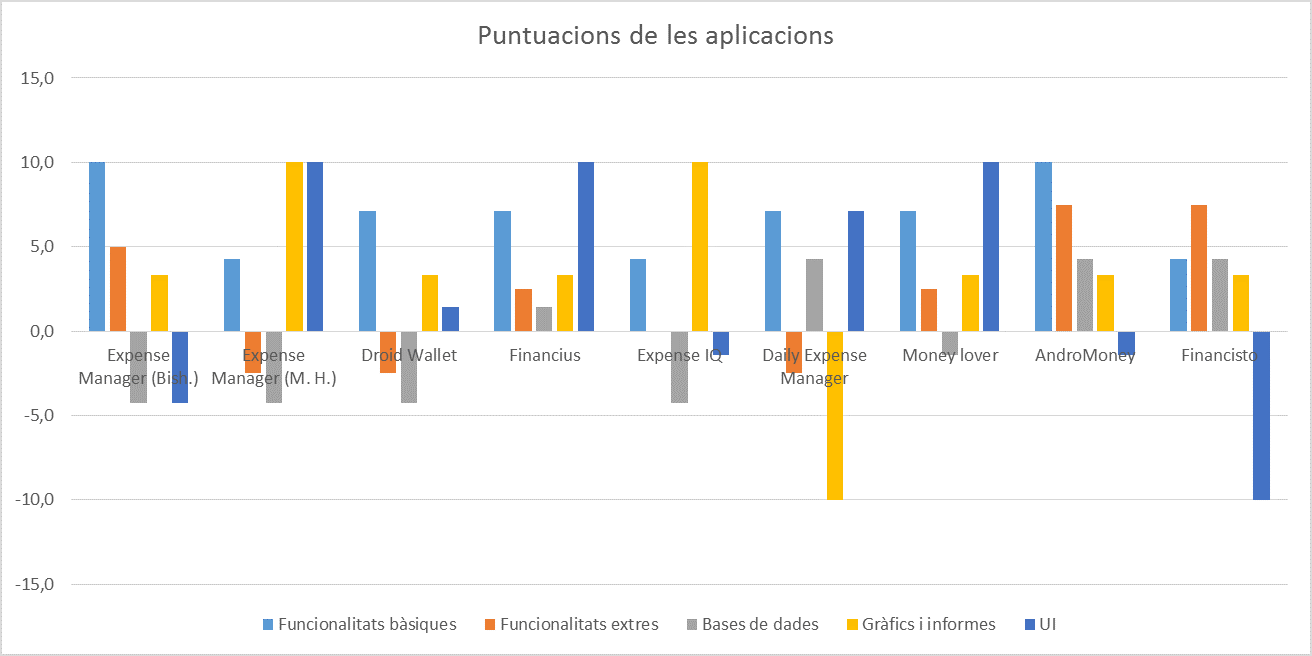
\includegraphics[scale=0.5]{grafic_apps.png}
\caption{Caracteristiques i funcions de les aplicacions per enregistrar despeses}\label{fig:taula_resum_apps}
\end{figure}

\subsection{Aplicacions per gestionar despeses en grup}
